\documentclass[11pt,a4paper]{article}

\usepackage{amsmath}
\usepackage{amssymb}
\usepackage{geometry}
\usepackage{graphicx}
\usepackage{placeins}
\usepackage{ragged2e}
\usepackage[onehalfspacing]{setspace}
\parindent0.0em
\geometry{left=3cm,right=3cm, top=4cm}


\date{}

\author{Claudine Schwarzenbach and Zeynep Eyibak}

\title{House Prices and Walkability in the US}


\begin{document}

\maketitle

We estimate how home values in a zip code relate to the Walk Score and Bike Score of its city and to commute times, controlling for the number of bedrooms.\\
Data sources:
\begin{itemize}
    \item Zillow: home values (ZHVI) at zip code level by number of bedrooms. We convert all values to dollars of the latest month in the data using the FRED CPI (CPIAUCSL). The Zillow URL changes from time to time; if the download fails, update it in \texttt{Data\_Download.py}.
    \item Walk Score: city-level Walk, Transit and Bike Scores, scraped from walkscore.com and merged on city and state. Scores are available only for larger cities, so part of the zip codes remain unmatched.
    \item Census (ACS 2021, 5-year): householder demographics (S2502) and travel time to work (B08303) at ZCTA level. ZCTAs approximate zip codes, so a small share of zip codes does not match.
\end{itemize}

\begin{figure}[h]
    \centering
    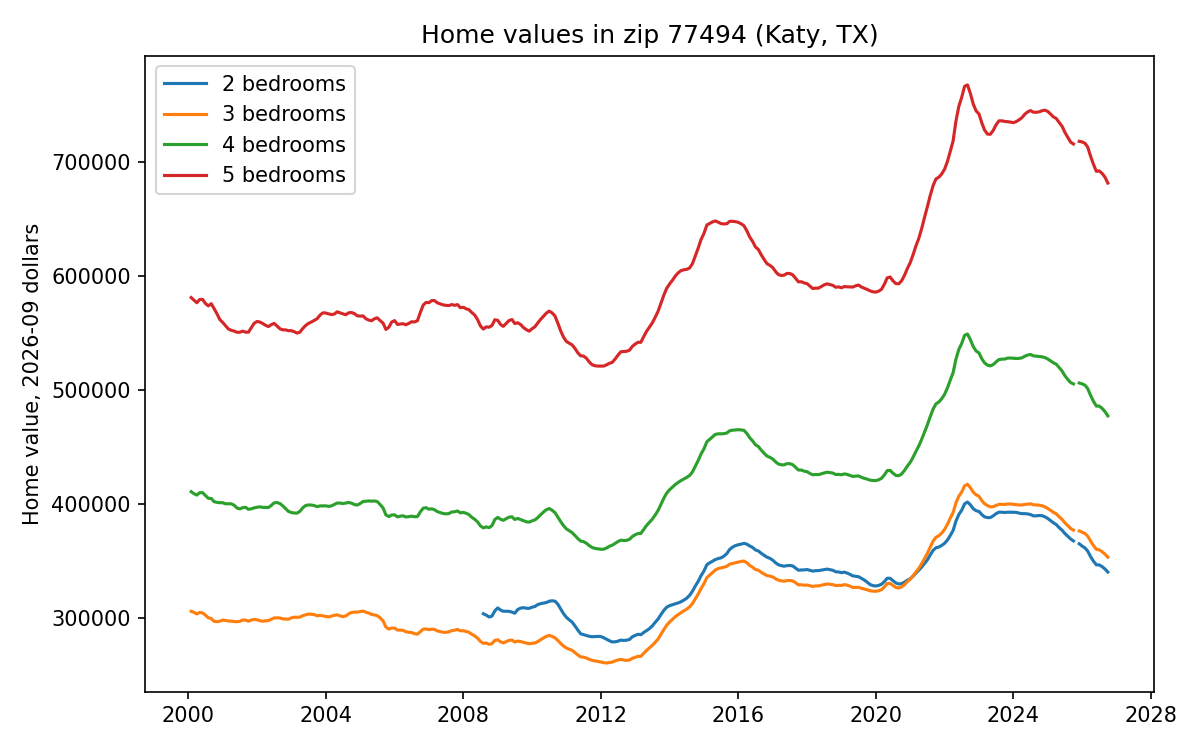
\includegraphics[width=0.8\textwidth]{Plots/Prices.png}
\end{figure}

\begin{figure}[h]
    \centering
    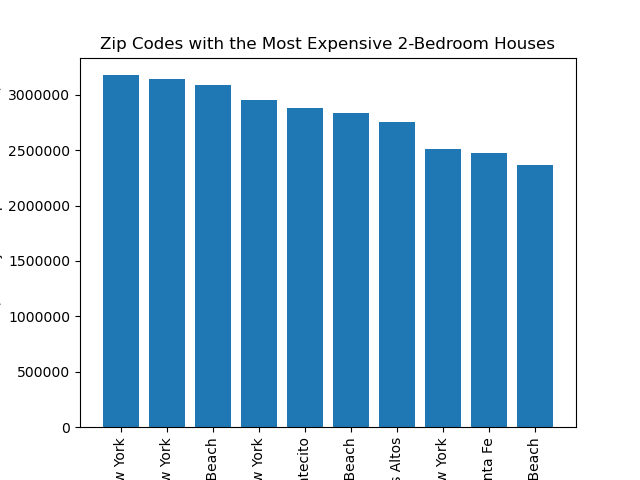
\includegraphics[width=0.8\textwidth]{Plots/Expensive.png}
\end{figure}

\begin{figure}[h]
    \centering
    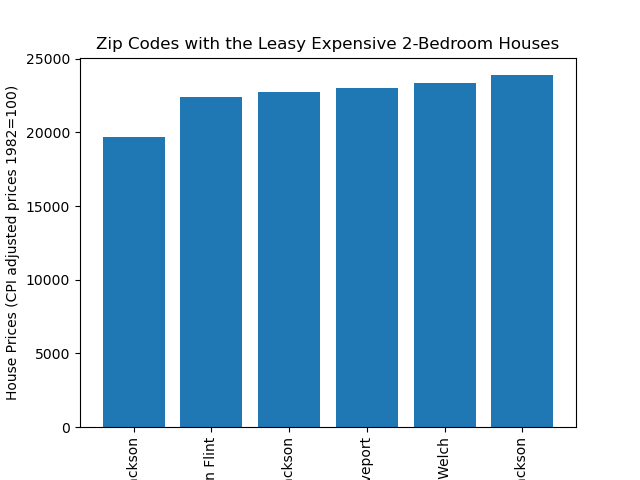
\includegraphics[width=0.8\textwidth]{Plots/Cheap.png}
\end{figure}

\FloatBarrier

\begin{figure}[h]
    \centering
    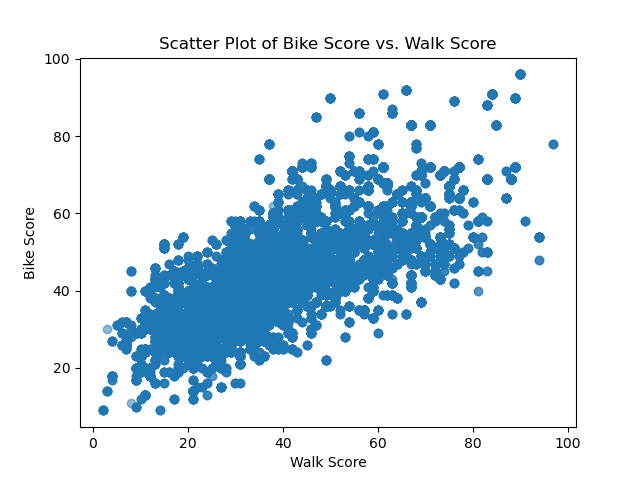
\includegraphics[width=0.6\textwidth]{Plots/Walk_Bike.png}
\end{figure}

\begin{figure}[h]
    \centering
    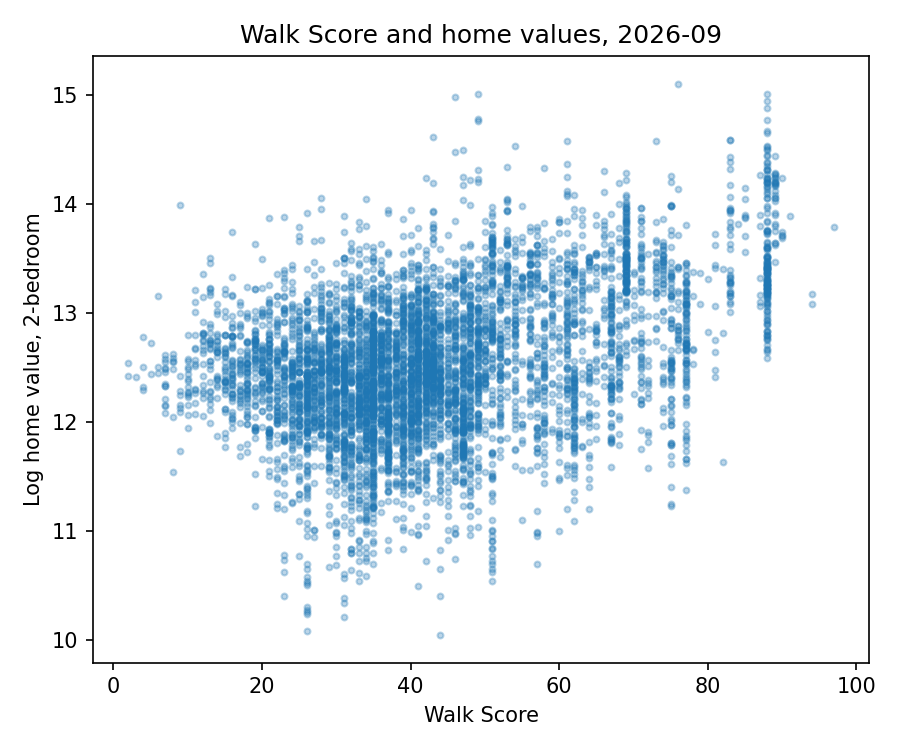
\includegraphics[width=0.6\textwidth]{Plots/Walk_Price.png}
\end{figure}

\begin{figure}[h]
    \centering
    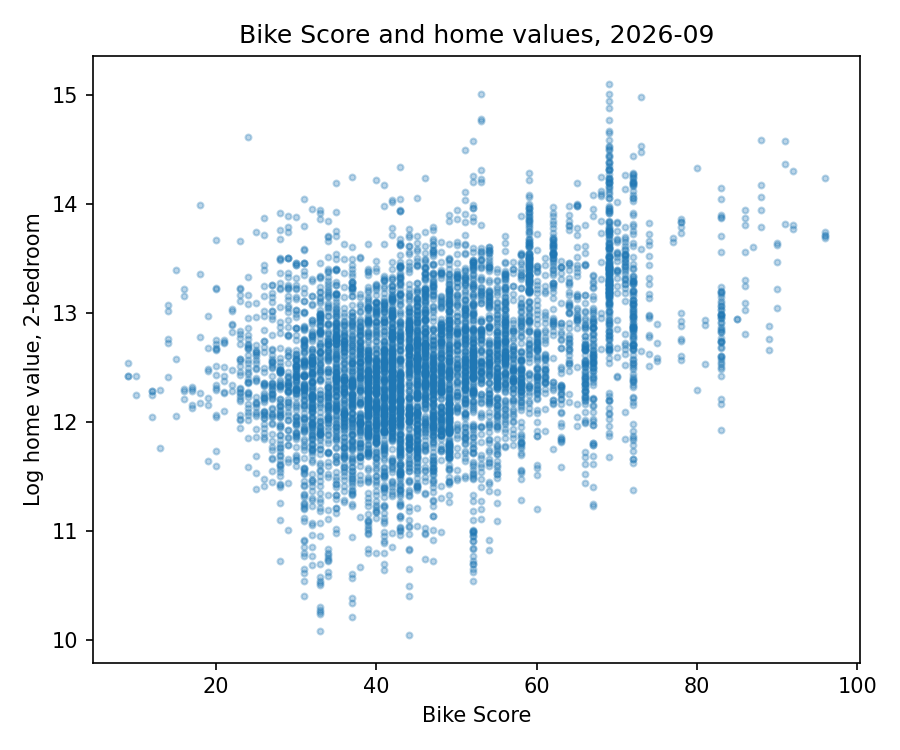
\includegraphics[width=0.6\textwidth]{Plots/Bike_Price.png}
\end{figure}

\FloatBarrier
\newpage
The regressions use one observation per zip code and number of bedrooms in the latest month of the data. The dependent variable is the log home value. All models include bedroom fixed effects. Walk and Bike Scores are measured at the city level, so standard errors are clustered by city.

\input{Tables/summary_1.tex}

\FloatBarrier
Commute shares are the percentage of workers in the zip code with a commute under 15 minutes (short) and of 40 minutes or more (long); 15 to 39 minutes is the omitted category.

\input{Tables/summary_2.tex}

\FloatBarrier
State fixed effects restrict the comparison to cities within the same state.

\input{Tables/summary_3.tex}


\end{document}
